\section{Triple Integrals}

\subsection{Interpretations of Triple Integrals}

Let $\mathcal{W} \subseteq \mathbb{R}^3$ be a solid region and let $f(x,y,z)$ be integrable on $\mathcal{W}$. The triple integral
\[
    \wiiint{f(x,y,z)}
\]
has several important interpretations:
\begin{enumerate}
    \item If $f$ is a density function with units of amount per unit volume, then
    \[
        \wiiint{f(x,y,z)}
    \]
    is the total amount contained in $\mathcal{W}$. In particular, if $f = \rho$ is a mass density, then the integral gives the mass of the solid.

    \item Taking $f = 1$ gives the volume of the region:
    \[
        \operatorname{Vol}(\mathcal{W}) = \wiiint{1}.
    \]

    \item The average value of $f$ over $\mathcal{W}$ is
    \[
        f_{\mathrm{avg}}
        = \frac{1}{\operatorname{Vol}(\mathcal{W})}
        \wiiint{f(x,y,z)}.
    \]

    \item Geometrically,
    \[
        \wiiint{f(x,y,z)}
    \]
    can be viewed as the signed hypervolume of the four-dimensional region determined by the graph of $f$ over $\mathcal{W}$.
\end{enumerate}

\subsection{Evaluating Triple Integrals}

As with double integrals, a triple integral may be approximated by a Riemann sum or evaluated exactly by writing it as an iterated integral.

\begin{theorem}{Fubini's Theorem for Triple Integrals}{fubini_triple}
If $f$ is continuous on the box
\[
    \mathcal{B} = [a,b] \times [c,d] \times [p,q],
\]
then
\[
    \xiiint{\mathcal{B}}{f(x,y,z)}
    = \int_a^b\int_c^d\int_p^q f(x,y,z)\,\dd{z}\,\dd{y}\,\dd{x}.
\]
The same conclusion holds for any of the other five orders of integration.

More generally, suppose $\mathcal{W}$ lies over a domain $\mathcal{D}$ in the $xy$-plane and is bounded below and above by $z = z_1(x,y)$ and $z = z_2(x,y)$, respectively. Then
\[
    \wiiint{f(x,y,z)}
    = \diint{\left(\int_{z_1(x,y)}^{z_2(x,y)}
    f(x,y,z)\,\dd{z}\right)}.
\]
\end{theorem}

\begin{example}[Volume of a Tetrahedron]
The plane $x + y + z = 1$ cuts off a tetrahedron $\mathcal{W}$ in the first octant. Describe $\mathcal{W}$ using inequalities in rectangular coordinates, then find its volume.
\end{example}

\begin{center}
\begin{tikzpicture}[
    scale=3,
    x={(1cm,-0.25cm)},
    y={(0.75cm,0.35cm)},
    z={(0cm,1cm)},
    >=Stealth
]
    % Define the vertices of the tetrahedron
    \coordinate (O) at (0,0,0);
    \coordinate (X) at (1,0,0);
    \coordinate (Y) at (0,1,0);
    \coordinate (Z) at (0,0,1);

    % Draw the coordinate axes
    \draw[->] (O) -- (1.25,0,0) node[below] {$x$};
    \draw[->] (O) -- (0,1.25,0) node[right] {$y$};
    \draw[->] (O) -- (0,0,1.25) node[above] {$z$};

    % Shade the four faces
    \filldraw[fill=orange!25, draw=orange!80!black, opacity=0.8] (O) -- (X) -- (Y) -- cycle;
    \filldraw[fill=orange!35, draw=orange!80!black, opacity=0.75] (O) -- (X) -- (Z) -- cycle;
    \filldraw[fill=orange!45, draw=orange!80!black, opacity=0.7] (O) -- (Y) -- (Z) -- cycle;
    \filldraw[fill=orange!55, draw=orange!90!black, opacity=0.65] (X) -- (Y) -- (Z) -- cycle;

    % Mark the intercepts
    \node[below] at (X) {$1$};
    \node[right] at (Y) {$1$};
    \node[left] at (Z) {$1$};
\end{tikzpicture}
\end{center}

\begin{sol}
Because $\mathcal{W}$ lies in the first octant and below the plane $z = 1 - x - y$,
\[
    \mathcal{W}
    = \{(x,y,z):x \geq 0,\ y \geq 0,\ z \geq 0,\ x + y + z \leq 1\}.
\]
Using the order $\dd{z}\,\dd{y}\,\dd{x}$, the bounds are
\[
    0 \leq x \leq 1,\qquad
    0 \leq y \leq 1 - x,\qquad
    0 \leq z \leq 1 - x - y.
\]
Therefore,
\begin{align*}
    \operatorname{Vol}(\mathcal{W})
    &= \int_0^1\int_0^{1 - x}\int_0^{1 - x - y}1\,\dd{z}\,\dd{y}\,\dd{x}\\
    &= \int_0^1\int_0^{1 - x}(1 - x - y)\,\dd{y}\,\dd{x}\\
    &= \frac{1}{2}\int_0^1(1 - x)^2\,\dd{x}
    = \frac{1}{6}.
\end{align*}
\end{sol}

\begin{example}[Mass Between Two Surfaces]
Let $\mathcal{W}$ be the solid bounded by $z = 1$, $z = 2 - y^2$, $x = 0$, and $x = 1$. The density at $(x,y,z)$ is $f(x,y,z)$ kilograms per cubic meter. Write an iterated integral for the mass of $\mathcal{W}$.
\end{example}

\begin{center}
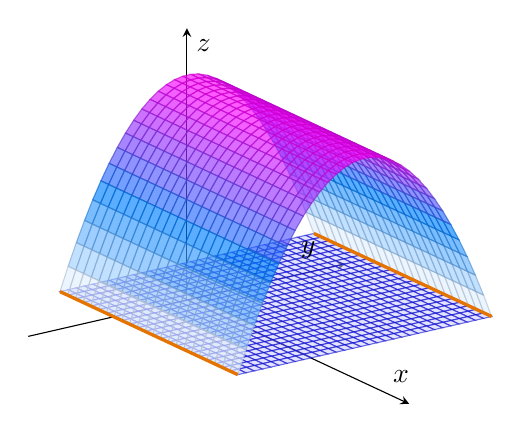
\begin{tikzpicture}
\begin{axis}[
    view={55}{25},
    axis lines=center,
    xlabel={$x$},
    ylabel={$y$},
    zlabel={$z$},
    xmin=0, xmax=1.25,
    ymin=-1.25, ymax=1.25,
    zmin=0.8, zmax=2.25,
    ticks=none,
    samples=24,
    samples y=32,
    z buffer=sort
]
    % Draw the lower plane
    \addplot3[
        surf,
        domain=0:1,
        domain y=-1:1,
        fill=blue!20,
        draw=blue!45,
        opacity=0.55
    ] {1};

    % Draw the upper parabolic cylinder
    \addplot3[
        surf,
        domain=0:1,
        domain y=-1:1,
        colormap/cool,
        opacity=0.65
    ] {2 - y^2};

    % Draw the intersection curves
    \addplot3[orange!90!black, very thick, domain=0:1, samples=2]
    (x,1,1);
    \addplot3[orange!90!black, very thick, domain=0:1, samples=2]
    (x,-1,1);
\end{axis}
\end{tikzpicture}
\end{center}

\begin{sol}
The two $z$-surfaces intersect when
\[
    1 = 2 - y^2 \iff y = \pm 1.
\]
Thus
\[
    \mathcal{W}
    = \{(x,y,z):0 \leq x \leq 1,\ -1 \leq y \leq 1,\ 1 \leq z \leq 2 - y^2\}.
\]
The mass is
\[
    M = \int_0^1\int_{-1}^1\int_1^{2 - y^2}
    f(x,y,z)\,\dd{z}\,\dd{y}\,\dd{x}.
\]
\end{sol}

\begin{example}[Choosing an Order of Integration]
Let $\mathcal{W}$ be the solid in the first octant bounded by
\[
    z = 4 - y^2,\qquad y = 2x,\qquad z = 0,\qquad x = 0.
\]
Calculate
\[
    \wiiint{xyz}.
\]
\end{example}

The three coordinate-plane projections of $\mathcal{W}$ are shown below.

\begin{center}
\begin{minipage}[t]{0.31\textwidth}
\centering
\textbf{Projection onto the $xy$-plane}

\begin{tikzpicture}[x=1.8cm,y=1.1cm,>=Stealth]
    % Shade the triangular projection
    \fill[orange!25] (0,0) -- (0,2) -- (1,2) -- cycle;
    \draw[orange!80!black, thick] (0,0) -- (0,2) -- (1,2) -- cycle;

    % Draw axes and labels
    \draw[->] (0,0) -- (1.3,0) node[right] {$x$};
    \draw[->] (0,0) -- (0,2.35) node[above] {$y$};
    \node[right] at (0.53,1.05) {\scriptsize $y = 2x$};
    \node[left] at (0,2) {\scriptsize $2$};
    \node[below] at (1,0) {\scriptsize $1$};
\end{tikzpicture}
\end{minipage}\hfill
\begin{minipage}[t]{0.31\textwidth}
\centering
\textbf{Projection onto the $yz$-plane}

\begin{tikzpicture}[x=1.05cm,y=0.55cm,>=Stealth]
    % Shade the region below the parabola
    \fill[blue!20]
    (0,0) -- plot[domain=0:2,samples=60] (\x,{4 - \x*\x}) -- cycle;
    \draw[blue!75!black, thick]
    plot[domain=0:2,samples=60] (\x,{4 - \x*\x});

    % Draw axes and labels
    \draw[->] (0,0) -- (2.35,0) node[right] {$y$};
    \draw[->] (0,0) -- (0,4.55) node[above] {$z$};
    \node[rotate=-45] at (1.18,2.15) {\scriptsize $z = 4 - y^2$};
    \node[left] at (0,4) {\scriptsize $4$};
    \node[below] at (2,0) {\scriptsize $2$};
\end{tikzpicture}
\end{minipage}\hfill
\begin{minipage}[t]{0.31\textwidth}
\centering
\textbf{Projection onto the $xz$-plane}

\begin{tikzpicture}[x=2.1cm,y=0.55cm,>=Stealth]
    % Shade the region below the projected parabola
    \fill[green!20]
    (0,0) -- plot[domain=0:1,samples=60] (\x,{4 - 4*\x*\x}) -- cycle;
    \draw[green!60!black, thick]
    plot[domain=0:1,samples=60] (\x,{4 - 4*\x*\x});

    % Draw axes and labels
    \draw[->] (0,0) -- (1.2,0) node[right] {$x$};
    \draw[->] (0,0) -- (0,4.55) node[above] {$z$};
    \node[rotate=-58] at (0.55,2.3) {\scriptsize $z = 4 - 4x^2$};
    \node[left] at (0,4) {\scriptsize $4$};
    \node[below] at (1,0) {\scriptsize $1$};
\end{tikzpicture}
\end{minipage}
\end{center}

\begin{sol}
The projection onto the $xy$-plane is
\[
    D_{xy}
    = \{(x,y):0 \leq y \leq 2,\ 0 \leq x \leq \tfrac{y}{2}\}.
\]
For each $(x,y)\in D_{xy}$, the variable $z$ ranges from the $xy$-plane to the parabolic cylinder:
\[
    0 \leq z \leq 4 - y^2.
\]
Therefore,
\begin{align*}
    \wiiint{xyz}
    &= \int_0^2\int_0^{y/2}\int_0^{4 - y^2}
    xyz\,\dd{z}\,\dd{x}\,\dd{y}\\
    &= \int_0^2\int_0^{y/2}
    \frac{xy}{2}(4 - y^2)^2\,\dd{x}\,\dd{y}\\
    &= \frac{1}{16}\int_0^2y^3(4 - y^2)^2\,\dd{y}.
\end{align*}
With $u = y^2$, so that $y^3\,\dd{y} = \frac{u}{2}\,\dd{u}$,
\begin{align*}
    \wiiint{xyz}
    &= \frac{1}{32}\int_0^4u(4 - u)^2\,\dd{u}\\
    &= \frac{2}{3}.
\end{align*}
\end{sol}
